\documentclass[conference,compsoc]{IEEEtran}


% *** CITATION PACKAGES ***
%
\ifCLASSOPTIONcompsoc
  % IEEE Computer Society needs nocompress option
  % requires cite.sty v4.0 or later (November 2003)
  \usepackage[nocompress]{cite}
\else
  % normal IEEE
  \usepackage{cite}
\fi
% cite.sty was written by Donald Arseneau
% V1.6 and later of IEEEtran pre-defines the format of the cite.sty package
% \cite{} output to follow that of the IEEE. Loading the cite package will
% result in citation numbers being automatically sorted and properly
% "compressed/ranged". e.g., [1], [9], [2], [7], [5], [6] without using
% cite.sty will become [1], [2], [5]--[7], [9] using cite.sty. cite.sty's
% \cite will automatically add leading space, if needed. Use cite.sty's
% noadjust option (cite.sty V3.8 and later) if you want to turn this off
% such as if a citation ever needs to be enclosed in parenthesis.
% cite.sty is already installed on most LaTeX systems. Be sure and use
% version 5.0 (2009-03-20) and later if using hyperref.sty.
% The latest version can be obtained at:
% http://www.ctan.org/pkg/cite
% The documentation is contained in the cite.sty file itself.
%
% Note that some packages require special options to format as the Computer
% Society requires. In particular, Computer Society  papers do not use
% compressed citation ranges as is done in typical IEEE papers
% (e.g., [1]-[4]). Instead, they list every citation separately in order
% (e.g., [1], [2], [3], [4]). To get the latter we need to load the cite
% package with the nocompress option which is supported by cite.sty v4.0
% and later.





% *** GRAPHICS RELATED PACKAGES ***
%
\ifCLASSINFOpdf
  % \usepackage[pdftex]{graphicx}
  % declare the path(s) where your graphic files are
  % \graphicspath{{../pdf/}{../jpeg/}}
  % and their extensions so you won't have to specify these with
  % every instance of \includegraphics
  % \DeclareGraphicsExtensions{.pdf,.jpeg,.png}
\else
  % or other class option (dvipsone, dvipdf, if not using dvips). graphicx
  % will default to the driver specified in the system graphics.cfg if no
  % driver is specified.
  % \usepackage[dvips]{graphicx}
  % declare the path(s) where your graphic files are
  % \graphicspath{{../eps/}}
  % and their extensions so you won't have to specify these with
  % every instance of \includegraphics
  % \DeclareGraphicsExtensions{.eps}
\fi


% correct bad hyphenation here
\hyphenation{op-tical net-works semi-conduc-tor}

\usepackage{cite}
%\usepackage{natbib}
\usepackage{amsmath}
\usepackage[pdftex]{graphicx}


%\usepackage{url,apacite}    % package url to prevent horrible linebreaks

\begin{document}

%
% paper title
% Titles are generally capitalized except for words such as a, an, and, as,
% at, but, by, for, in, nor, of, on, or, the, to and up, which are usually
% not capitalized unless they are the first or last word of the title.
% Linebreaks \\ can be used within to get better formatting as desired.
% Do not put math or special symbols in the title.
\title{Combining Q-Learning with Artificial Neural Networks in Flappy Bird
\\ Project Report of COMP 599}


% author names and affiliations
% use a multiple column layout for up to three different
% affiliations
\author{\IEEEauthorblockN{Jianan Yue}
\IEEEauthorblockA{
McGill University\\
Montreal, Quebec H3A0C3\\
Email: jianan.yue@mail.mcgill.ca}
\and
\IEEEauthorblockN{Yulin Shi}
\IEEEauthorblockA{McGill University\\
Montreal, Quebec H3A0C3\\
Email: yulin.shi@mail.mcgill.ca}
}
% make the title area
\maketitle

% As a general rule, do not put math, special symbols or citations
% in the abstract
\begin{abstract}
For the flappy bird game, a typical delay control problem, we propose using the reinforcement learning algorithms to learn the control policy. Specifically, we use the Bellman equation to propagate the end-point reward to the entire state space; use model free Q-function to search optimal policy; and, to deal with the curse of dimension, use the neural network to parametrise the approximate function of the optimal controller. The Flappy Bird environment is developed in the JavaScript. The open source machine learning library Convnetjs is included to train the neural network. It is validated that the neural network Q-learning is proper for the learning problem. It is also observed that some strategies emerged after training the simple neural network.
\end{abstract}

% no keywords




% For peer review papers, you can put extra information on the cover
% page as needed:
% \ifCLASSOPTIONpeerreview
% \begin{center} \bfseries EDICS Category: 3-BBND \end{center}
% \fi
%
% For peerreview papers, this IEEEtran command inserts a page break and
% creates the second title. It will be ignored for other modes.
\IEEEpeerreviewmaketitle



\section{Introduction}
% no \IEEEPARstart

% You must have at least 2 lines in the paragraph with the drop letter
% (should never be an issue)


\subsection{Flappy Bird Problem}
The well-known game Flappy bird, in a functional perspective of view, is a simulation world consists with a part of deterministic dynamic: the acceleration and a part of stochastic dynamic: the position of the gap. By observing the location of the path and estimating the trajectory of the bird in a continuous time, the players selects among two input commands. The object is to go through as many gaps as possible while avoiding colliding with the pipes.  The game can be described in discrete time as a Markov process. 
\begin{equation}
s' \sim \varepsilon (s,a)
\end{equation}
where $s$ is the current state, $a$ is the current action, $s'$ is the next state. Symbol $\sim$ mean the value of $s'$ is subject to a distribution. 

In this view, it is feasible to use an artificial agent following a policy \eqref{eq:flappyPolicy} such as the $\epsilon$-greedy policy to replace human as the player to play the Flappy Bird game. \cite{sutton1998reinforcement} 
\begin{equation}\label{eq:flappyPolicy}
a=\pi(s)
\end{equation}

\subsection{Reinforcement Learning}
One difficulty of learning the Flappy Bird problem is that the leaner agent does not perceive a prompt reward after taking an action. Rather, they get the reward at the end of an episode which is defined as the entire state-action trajectory of a round of play. At the end of an episode, the reward is proportional to the number of pipes the bird goes through. The agent is trained to learn a policy that maximize the overall reward. 
However, the strong delayed reward in the Flappy Bird problem invalids the classical machine learning algorithms such as the regression and classification which assumes that the samples are independent. For example, the agent does not perceive any reward or penalty when it does not choose the jump action and stays far away from the gap, even if these actions and states have a strong negative influence on the subsequent rewards. Therefore, we need an index that reflect the expected utility of a state, other than the instantaneous reward. We call the index as the value function
\begin{equation}\label{eq:rlValue}
V^{\pi}(s)
= E_{\pi} \left\{ R_t | s_t =s \right\}
= E_{\pi} \left\{ \sum_{k=0}^{\infty} \gamma^k r_{t+k+1} | s_t =s \right\}
\end{equation}
where $0<\gamma\leq 1$ is the discount factor. 
 
For the Flappy Bird problem as a Markov process, the definition of the \eqref{eq:rlValue} can be reformulated as the Bellman equation \eqref{eq:bellman} and solved using episode samples iteratively. 
\begin{equation}\label{eq:bellman}
V^{\pi}(s)
= E_{\pi} \left\{ r_{t+1}+\gamma V^{\pi}(s_{t+1}) | s_t =s \right\}
\end{equation}

For a time-invariant system with smooth value function, the iterative equation \eqref{eq:rlValue} is a contraction map. The value function will converge to its fixed point. 

\subsection{Q-learning}
Another issue arising is that while the value function alone does not tell the agent how to act without a model \eqref{eq:valueModel} which can be very complex in real environments and usually suffers greatly from poor accuracy. ~\cite{strehl2006pac}
\begin{equation}\label{eq:valueModel}
\hat{s}' = \hat{\varepsilon} (s,a)
\end{equation}

Since the Flappy Bird problem is basically a control problem, it is worthy of considering a model-free approach. Here we first define a $Q$ function with respect to state and action 
\begin{equation}
Q^{\pi} (s,a) = E_{\pi} \left\{ r_{t+1} +\gamma V^{\pi}(s_{t+1}) | s_t =s, a_t=a\right\}
\end{equation}
Given the value of a $Q$ function, it is possible to generate an optimal policy without a model
\begin{equation}
\pi(s) \leftarrow \arg \max_{a\in \mathcal{A}} Q(s,a)
\end{equation}

There are basically two approaches of learning the $Q$ function given episode samples: off-policy \eqref{eq:qlearningOff} where actions are chosen greedily and on-policy (SARSA) \eqref{eq:qlearningOn} where actions are chosen based on the policy.
\begin{equation}\label{eq:qlearningOff}
Q(s,a) \leftarrow Q(s,a) + \alpha \left(r+\gamma \max_{a'} Q(s',a')-Q(s,a) \right)
\end{equation}
\begin{equation}\label{eq:qlearningOn}
Q(s,a) \leftarrow Q(s,a) + \alpha \left(r+\gamma Q(\pi(s,a),a')-Q(s,a) \right)
\end{equation}

\subsection{Artificial Neural Network}
For low dimensional problem, is it feasible to use tables to describe the value functions of discrete states. However, for large dimensional problems like the Flappy Bird problem, due to the curse of dimension, the table of the value function can be very large, which makes it impractical to maintain and retrieve. In this case, a good alternative might be to use parametrized function to approximate the policy function. 

Function approximation falls into two categories: linear function approximation and nonlinear function approximation. In a linear function approximation, the value of function is the linear combination of a set of nonlinear feature functions like the polynomial function, Gaussian function and other customized functions. Good understanding of the model is needed for choosing good feature functions. Nonlinear function approximation includes search tree, neural network etc. They are found to be able to learn complex problems adaptively. Therefore, in this project, we choose the neural network to parameterize the policy function. 

%%%%%%%%%%%%%%%%%%%%%%%%%%%%%%%%%%%%%%%%%%%%%%%%%%%%%%%%%%%%%%%%%%%%%%%%%%%%%%%%%%%%%%%%%%
\section{Software Architecture}
%%%%%%%%%%%%%%%%%%%%%%%%%%%%%%%%%%%%%%%%%%%%%%%%%%%%%%%%%%%%%%%%%%%%%%%%%%%%%%%%%%%%%%%%%%
\begin{figure}[!t]
\centering
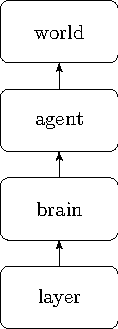
\includegraphics[width=0.6in]{softwareArchitecture}
\caption{Software Architecture}
\label{softwareArchitecture}
\end{figure}
For the simulation and learning task of the project, a three level object-oriented programming architecture is designed in JavaScript: the ``World'', the ``Agent'', the ``Brain (neural network)'' and the ``Layer''. A world supports stochastic environment simulations. It calls an agent object and sends it the partially observed states. The relationship is in Figure \ref{softwareArchitecture}. 

In each time step, the world and the agent is updated according to the action and the previous state. the agent calls a brain, passes the state and reward to the brain and obtain the action command from the brain. The brain calls the layers for Q-function values. 

\subsection{Layer}
There are different types of layers. Each uses a different excitation function like sigmoid functions, tanh functions, relu functions and maxout functions. The number of neurons can be customized by users during layer construction. 

The connected layers are not expected to be able to select from a set of admissible actions for the agent directly. In stead, they together estimate the value of the Q-function whose value will be passed to the brain. Therefore, the output layer becomes special because it produces the value function while the output value of intermediate layers are meaningless. The common feature of all layers is that they all define ``forward'' functions which make prediction and ``backward'' function which updates layer parameters. 

\subsection{Brain}
A ``Brain'' class has layer attributes. The users define the layers depth, layer types and the initial parameters of the neuron layers. Actions of an agent is selected in the ``forward'' function of a brain. It either chooses among all actions the one corresponds to the best value, or in a small probability, chooses an action in a random distribution. The later is called the $\epsilon$-greedy policy. The $\epsilon$-greedy policy allows the agent to explore the environment. 

\subsection{Agent} 
An agent object (which is a bird in the game) stores its current state. It update its height, distance and velocity states according to the Newton's law and the action. It serves as the deterministic part of the environment. Each agent has a brain. We define distance to the gap as heuristic rewards in addition to the final rewards, for helping boosting the training speed. 

\subsection{World}
The stochastic environment is created in the ``World'' class. It creates a new pipe when the ``bird'' flies through a pair of pipe. The heigh of the gap of the pipe is chosen in random, which serves as the unknown part of the environment. Collision is detected in the world and passed to the agent. 

\section{Experiments}


\section{Results and Discussions}


% An example of a floating figure using the graphicx package.
% Note that \label must occur AFTER (or within) \caption.
% For figures, \caption should occur after the \includegraphics.
% Note that IEEEtran v1.7 and later has special internal code that
% is designed to preserve the operation of \label within \caption
% even when the captionsoff option is in effect. However, because
% of issues like this, it may be the safest practice to put all your
% \label just after \caption rather than within \caption{}.
%
% Reminder: the "draftcls" or "draftclsnofoot", not "draft", class
% option should be used if it is desired that the figures are to be
% displayed while in draft mode.
%
%\begin{figure}[!t]
%\centering
%\includegraphics[width=2.5in]{myfigure}
% where an .eps filename suffix will be assumed under latex, 
% and a .pdf suffix will be assumed for pdflatex; or what has been declared
% via \DeclareGraphicsExtensions.
%\caption{Simulation results for the network.}
%\label{fig_sim}
%\end{figure}

% Note that the IEEE typically puts floats only at the top, even when this
% results in a large percentage of a column being occupied by floats.


% An example of a double column floating figure using two subfigures.
% (The subfig.sty package must be loaded for this to work.)
% The subfigure \label commands are set within each subfloat command,
% and the \label for the overall figure must come after \caption.
% \hfil is used as a separator to get equal spacing.
% Watch out that the combined width of all the subfigures on a 
% line do not exceed the text width or a line break will occur.
%
%\begin{figure*}[!t]
%\centering
%\subfloat[Case I]{\includegraphics[width=2.5in]{box}%
%\label{fig_first_case}}
%\hfil
%\subfloat[Case II]{\includegraphics[width=2.5in]{box}%
%\label{fig_second_case}}
%\caption{Simulation results for the network.}
%\label{fig_sim}
%\end{figure*}
%
% Note that often IEEE papers with subfigures do not employ subfigure
% captions (using the optional argument to \subfloat[]), but instead will
% reference/describe all of them (a), (b), etc., within the main caption.
% Be aware that for subfig.sty to generate the (a), (b), etc., subfigure
% labels, the optional argument to \subfloat must be present. If a
% subcaption is not desired, just leave its contents blank,
% e.g., \subfloat[].


% An example of a floating table. Note that, for IEEE style tables, the
% \caption command should come BEFORE the table and, given that table
% captions serve much like titles, are usually capitalized except for words
% such as a, an, and, as, at, but, by, for, in, nor, of, on, or, the, to
% and up, which are usually not capitalized unless they are the first or
% last word of the caption. Table text will default to \footnotesize as
% the IEEE normally uses this smaller font for tables.
% The \label must come after \caption as always.
%
%\begin{table}[!t]
%% increase table row spacing, adjust to taste
%\renewcommand{\arraystretch}{1.3}
% if using array.sty, it might be a good idea to tweak the value of
% \extrarowheight as needed to properly center the text within the cells
%\caption{An Example of a Table}
%\label{table_example}
%\centering
%% Some packages, such as MDW tools, offer better commands for making tables
%% than the plain LaTeX2e tabular which is used here.
%\begin{tabular}{|c||c|}
%\hline
%One & Two\\
%\hline
%Three & Four\\
%\hline
%\end{tabular}
%\end{table}


% Note that the IEEE does not put floats in the very first column
% - or typically anywhere on the first page for that matter. Also,
% in-text middle ("here") positioning is typically not used, but it
% is allowed and encouraged for Computer Society conferences (but
% not Computer Society journals). Most IEEE journals/conferences use
% top floats exclusively. 
% Note that, LaTeX2e, unlike IEEE journals/conferences, places
% footnotes above bottom floats. This can be corrected via the
% \fnbelowfloat command of the stfloats package.




\section{Conclusion}
The conclusion goes here.




% conference papers do not normally have an appendix



% use section* for acknowledgment
\ifCLASSOPTIONcompsoc
  % The Computer Society usually uses the plural form
  \section*{Acknowledgments}
\else
  % regular IEEE prefers the singular form
  \section*{Acknowledgment}
\fi


The authors would like to thank...





% trigger a \newpage just before the given reference
% number - used to balance the columns on the last page
% adjust value as needed - may need to be readjusted if
% the document is modified later
%\IEEEtriggeratref{8}
% The "triggered" command can be changed if desired:
%\IEEEtriggercmd{\enlargethispage{-5in}}

% references section

% can use a bibliography generated by BibTeX as a .bbl file
% BibTeX documentation can be easily obtained at:
% http://mirror.ctan.org/biblio/bibtex/contrib/doc/
% The IEEEtran BibTeX style support page is at:
% http://www.michaelshell.org/tex/ieeetran/bibtex/
%\bibliographystyle{IEEEtran}
% argument is your BibTeX string definitions and bibliography database(s)
%\bibliography{IEEEabrv,../bib/paper}
%
% <OR> manually copy in the resultant .bbl file
% set second argument of \begin to the number of references
% (used to reserve space for the reference number labels box)
%\begin{thebibliography}{1}
%
%\bibitem{IEEEhowto:kopka}
%H.~Kopka and P.~W. Daly, \emph{A Guide to \LaTeX}, 3rd~ed.\hskip 1em plus
%  0.5em minus 0.4em\relax Harlow, England: Addison-Wesley, 1999.
%
%\end{thebibliography}

\bibliography{mybib.bib}{}
\bibliographystyle{plain}


% that's all folks
\end{document}


